\chapter{Jetpack Compose: Podstawy UI i Stanu (Wykład 9)}

Jetpack Compose to deklaratywny toolkit do budowania natywnego interfejsu użytkownika na Androida. Jego premiera (wersja 1.0 w 2021 roku) oznaczała największą rewolucję w tworzeniu UI od początku istnienia systemu.

Aby zrozumieć, dlaczego powstał Compose, musimy cofnąć się do roku 2008. Klasyczny system widoków (\textit{View System}), oparty na XML, towarzyszył Androidowi od wersji 1.0. Przez ponad dekadę ewoluował, ale dźwigał bagaż wczesnych decyzji projektowych:
\begin{enumerate}
    \item \textbf{Globalny stan i mutowalność}: W klasycznym podejściu programista musiał ręcznie zarządzać stanem widoku. Należało znaleźć widok (\texttt{findViewById}), a następnie wywołać metodę mutującą jego stan (np. \texttt{textView.setText()}). Prowadziło to często do błędów, gdy stan danych w aplikacji rozjeżdżał się ze stanem wyświetlanym na ekranie.
    \item \textbf{Dziedziczenie}: Klasa \texttt{View.java} ma obecnie ponad 30 000 linii kodu. Wszystkie komponenty dziedziczą po niej ogromną ilość funkcjonalności, której często nie potrzebują (np. \texttt{Button} dziedziczy po \texttt{TextView}).
    \item \textbf{Zależność od systemu}: Klasyczne widoki są częścią frameworka systemu Android (\texttt{android.jar}). Naprawienie błędu w \texttt{CheckBox} wymagało aktualizacji całego systemu operacyjnego u użytkownika.
\end{enumerate}

Jetpack Compose rozwiązuje te problemy, będąc biblioteką \textbf{niezależną od wersji systemu} (tzw. \textit{unbundled}). Możemy używać nowych funkcji UI nawet na starszych telefonach, po prostu aktualizując wersję biblioteki w projekcie.

\section{Imperatywny vs Deklaratywny Model UI}

Różnica między starym a nowym podejściem jest fundamentalna:

\begin{itemize}
    \item \textbf{Podejście Imperatywne (XML + View)}: Skupiamy się na tym, \textit{JAK} zmienić UI.
    \begin{minted}[fontsize=\small]{kotlin}
    // XML
    val button = findViewById<Button>(R.id.button)
    // Imperatywna zmiana stanu:
    button.setOnClickListener {
        button.text = "Kliknięto!"
        button.setBackgroundColor(Color.RED)
    }
    \end{minted}
    
    \item \textbf{Podejście Deklaratywne (Compose)}: Skupiamy się na tym, \textit{CO} ma zostać wyświetlone dla danego stanu.
    \begin{minted}[fontsize=\small]{kotlin}
    // Compose
    @Composable
    fun MyButton(isClicked: Boolean) {
        // UI jest funkcją stanu
        Button(
            colors = if (isClicked) Color.Red else Color.Blue
        ) {
            Text(if (isClicked) "Kliknięto!" else "Kliknij mnie")
        }
    }
    \end{minted}
\end{itemize}

W Compose nie \textit{zmieniamy} tekstu przycisku. My opisujemy interfejs na nowo dla nowych danych, a framework zajmuje się tym, by odświeżyć (\textit{zrekomponować}) tylko te elementy, które faktycznie uległy zmianie.

\section{Podstawowe Komponenty Layoutu}

W Jetpack Compose interfejs budujemy, składając ze sobą funkcje oznaczone adnotacją \texttt{@Composable}. Zamiast znanych z XML \texttt{LinearLayout} czy \texttt{FrameLayout}, używamy ich odpowiedników:

\texttt{Column} układa elementy w pionie (jeden pod drugim). Odpowiednik \texttt{LinearLayout} z orientacją pionową.

\begin{minted}[frame=single,framesep=10pt]{kotlin}
@Composable
fun ColumnExample() {
    Column {
        Text("Element 1 (Góra)")
        Text("Element 2 (Środek)")
        Text("Element 3 (Dół)")
    }
}
\end{minted}

\begin{figure}[h]
    \centering
    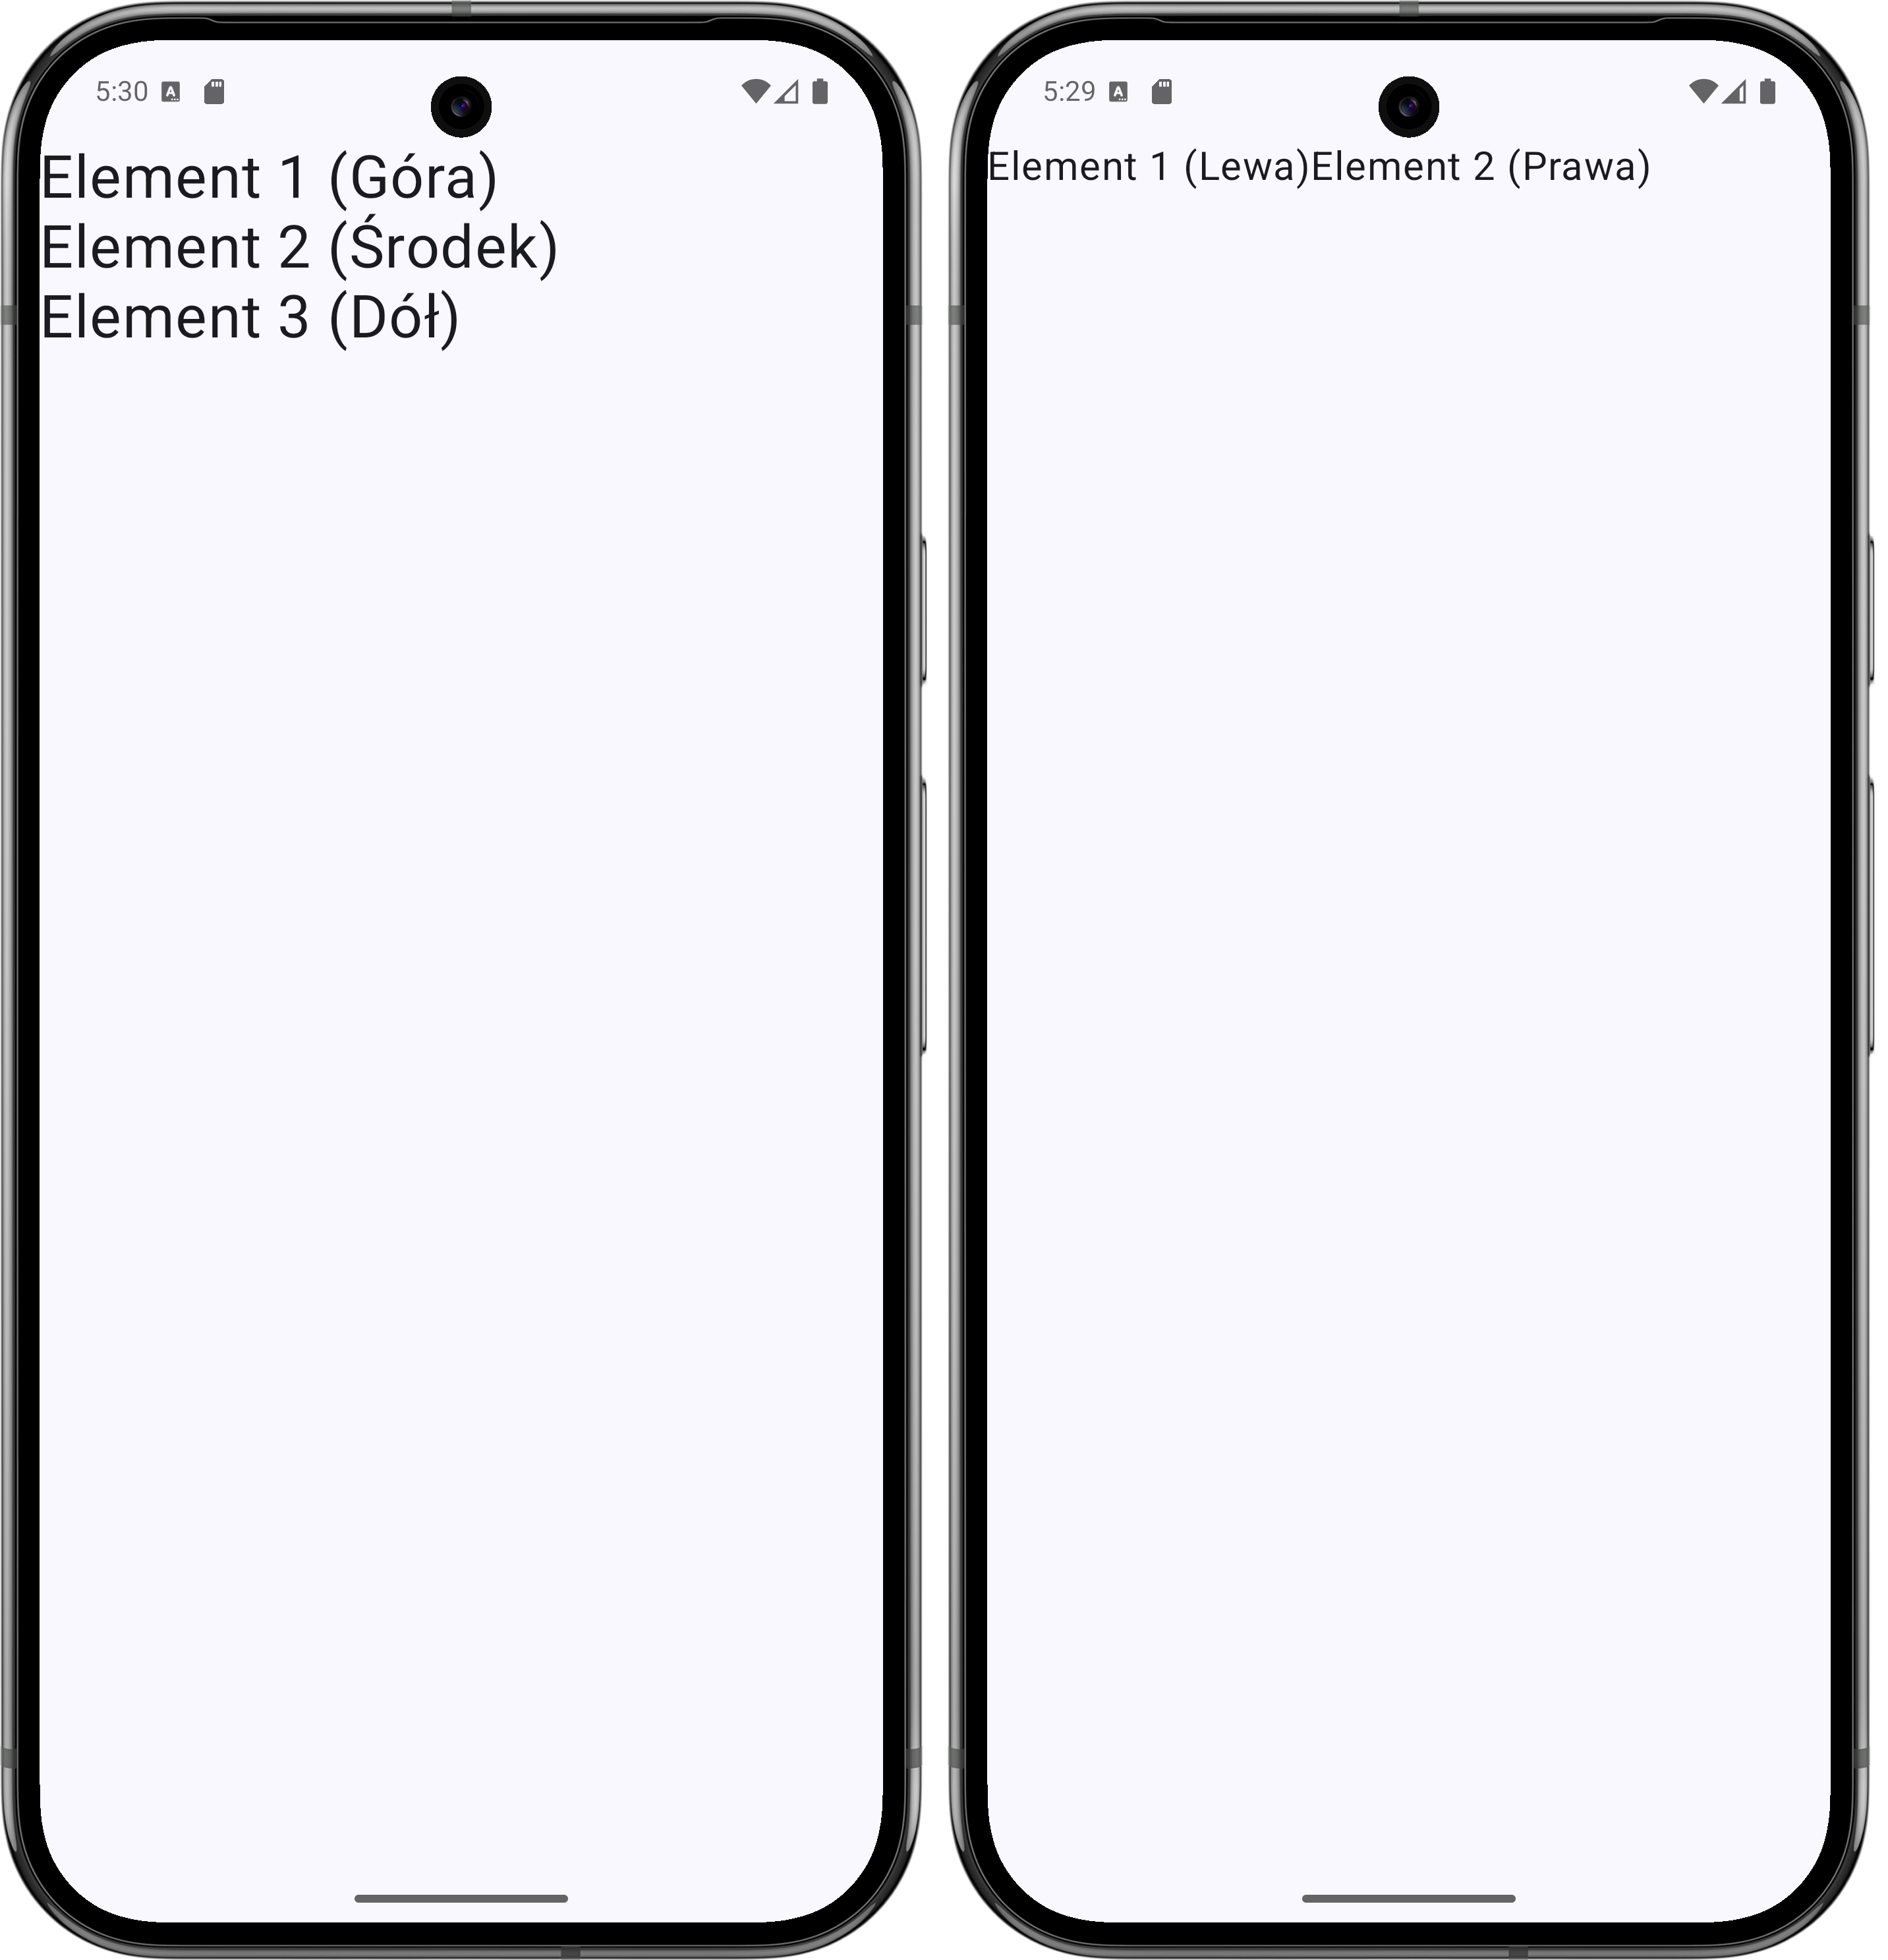
\includegraphics[width=0.4\textwidth]{fig/pum1-w09-column_row_example.png}
    \caption{Przykładowy layout z komponentem \texttt{Column} i \texttt{Row}}
    \label{fig:column_row_example}
\end{figure}

\texttt{Row} układa elementy w poziomie (jeden obok drugiego). Odpowiednik \texttt{LinearLayout} z orientacją poziomą.

\begin{minted}[frame=single,framesep=10pt]{kotlin}
@Composable
fun RowExample() {
    Row {
        Text("Lewa")
        Text("Prawa")
    }
}
\end{minted}

\texttt{Box} układa elementy jeden na drugim (warstwowo). Odpowiednik \texttt{FrameLayout}. Pierwszy element w kodzie ląduje na samym spodzie, a kolejne są rysowane na nim.

\begin{minted}[frame=single,framesep=10pt]{kotlin}
@Composable
fun BoxExample() {
    Box {
        Text("Tło (Pod spodem)")
        Text("Napis (Na wierzchu)")
    }
}
\end{minted}

Siłą Compose jest łatwość łączenia tych komponentów. Poniżej przykład prostego layoutu, gdzie elementy zewnętrzne są ułożone w poziomie, a elementy wewnętrzne w pionie.

\begin{minted}[frame=single,framesep=10pt]{kotlin}
@Composable
fun UserProfile(name: String) {
    Row {
        // Tekst po lewej
        Text(text = "A") 
        
        // Tekst po prawej, ułożony pionowo
        Column {
            Text("Witaj,")
            Text(name)
        }
    }
}
\end{minted}

Do wyświetlania tekstu służy komponent \texttt{Text}. Przy określaniu rozmiarów w Androidzie używamy dwóch jednostek:

\begin{itemize}
    \item \textbf{dp (density-independent pixels)}: Używane do wymiarów (marginesy, szerokość, wysokość). Zapewniają ten sam fizyczny rozmiar elementu na ekranach o różnej gęstości pikseli.
    \item \textbf{sp (scale-independent pixels)}: Używane \textbf{tylko do rozmiaru czcionki}. Działają jak \texttt{dp}, ale dodatkowo uwzględniają ustawienia systemowe użytkownika (np. powiększony tekst dla osób słabowidzących).
\end{itemize}

\section{Modyfikatory (Modifiers)}

\texttt{Modifier} to potężne narzędzie w Compose, które pozwala modyfikować wygląd i zachowanie komponentu (np. dodać tło, margines, obsługę kliknięcia).

Kluczową zasadą jest to, że modyfikatory działają \textbf{sekwencyjnie} (jak łańcuch). Kolejność wywołań ma znaczenie!

\begin{minted}[frame=single,framesep=10pt]{kotlin}
// Przykład: Kolejność paddingu i tła
Box(
    modifier = Modifier
        .background(Color.Red)   // 1. Najpierw czerwone tło
        .padding(16.dp)          // 2. Potem wcięcie (padding) wewnątrz czerwonego tła
        .background(Color.Blue)  // 3. Niebieskie tło wewnątrz paddingu
) {
    Text("Hej!")
}
\end{minted}

Gdybyśmy zamienili kolejność \texttt{padding} i \texttt{background}, efekt wizualny byłby zupełnie inny.

Najczęstsze modyfikatory:
\begin{itemize}
    \item \texttt{.fillMaxSize()}: Zajmij całą dostępną przestrzeń.
    \item \texttt{.padding()}: Odstęp wewnętrzny.
    \item \texttt{.clickable \{ \}}: Reakcja na dotyk.
\end{itemize}

\section{Układ i Wyrównanie (Alignment vs Arrangement)}

Rozmieszczanie elementów w kontenerach \texttt{Row} i \texttt{Column} opiera się na dwóch kluczowych pojęciach: \textbf{osi głównej} (Main Axis) i \textbf{osi poprzecznej} (Cross Axis).

\begin{itemize}
    \item \textbf{Arrangement (Rozmieszczenie)}: Kontroluje układ elementów wzdłuż \textbf{osi głównej}.
    \item \textbf{Alignment (Wyrównanie)}: Kontroluje układ elementów wzdłuż \textbf{osi poprzecznej}.
\end{itemize}

Oznacza to, że dostępne właściwości zależą od używanego kontenera:

\begin{table}[h]
\centering
\begin{tabular}{|c|c|c|}
\hline
\textbf{Kontener} & \textbf{Oś Główna (Arrangement)} & \textbf{Oś Poprzeczna (Alignment)} \\ \hline
\texttt{Column} & Pionowa (\texttt{verticalArrangement}) & Pozioma (\texttt{horizontalAlignment}) \\ \hline
\texttt{Row} & Pozioma (\texttt{horizontalArrangement}) & Pionowa (\texttt{verticalAlignment}) \\ \hline
\end{tabular}
\caption{Osie w kontenerach Row i Column}
\label{tab:axes}
\end{table}

Parametr \texttt{Arrangement} pozwala na precyzyjne określenie odstępów między elementami (dziećmi). Najpopularniejsze opcje to:

\begin{itemize}
    \item \texttt{Arrangement.Start} (dla Row) / \texttt{Top} (dla Column): Elementy \textit{przyklejone} do początku osi.
    \item \texttt{Arrangement.End} (dla Row) / \texttt{Bottom} (dla Column): Elementy \textit{przyklejone} do końca osi.
    \item \texttt{Arrangement.Center}: Elementy zgrupowane na środku osi, stykające się ze sobą.
    \item \texttt{Arrangement.SpaceBetween}: Pierwszy i ostatni element są przy krawędziach, a pozostała przestrzeń jest \textbf{równo} rozdzielona między nimi.
    \item \texttt{Arrangement.SpaceAround}: Podobnie jak SpaceBetween, ale dodaje odstęp również przed pierwszym i po ostatnim elemencie (połowa odstępu wewnętrznego).
    \item \texttt{Arrangement.SpaceEvenly}: Wszystkie odstępy (również te skrajne) są identycznej wielkości.
\end{itemize}

\begin{figure}[h]
    \centering
    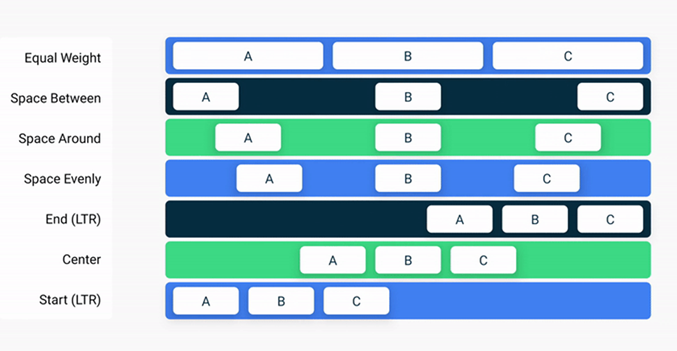
\includegraphics[width=0.8\textwidth]{fig/pum1-w09-arrangement.png}
    \caption{Wizualizacja opcji Arrangement: SpaceBetween, SpaceAround, SpaceEvenly}
    \label{fig:arrangement_viz}
\end{figure}

Czasami zamiast odstępów chcemy, aby element zajmował \textbf{proporcjonalną} część dostępnego miejsca. Służy do tego modyfikator \texttt{weight}.
Jeśli w \texttt{Row} mamy dwa elementy, oba z \texttt{.weight(1f)}, to podzielą one szerokość po równo (50\% / 50\%). Jeżeli chcemy zmienić proporcje, dostosowujemy wagi elementów.

\begin{minted}[frame=single,framesep=10pt]{kotlin}
Row(modifier = Modifier.fillMaxWidth()) {
    // Lewy element zajmie 1/3 (1f / (1f+2f))
    Box(Modifier.weight(1f).background(Color.Red))
    // Prawy element zajmie 2/3 (2f / (1f+2f))
    Box(Modifier.weight(2f).background(Color.Blue))
}
\end{minted}

Poniższy kod centruje element zarówno w pionie, jak i w poziomie. Zauważ, że nazwy parametrów są precyzyjne (\texttt{verticalArrangement} vs \texttt{horizontalAlignment}), co zapobiega pomyłkom.

\begin{minted}[frame=single,framesep=10pt]{kotlin}
Column(
    modifier = Modifier.fillMaxSize(),
    // Oś główna Column = Pionowa -> Arrangement
    verticalArrangement = Arrangement.Center, 
    // Oś poprzeczna Column = Pozioma -> Alignment
    horizontalAlignment = Alignment.CenterHorizontally 
) {
    Text("Na samym środku ekranu")
}
\end{minted}

\begin{figure}[h]
    \centering
    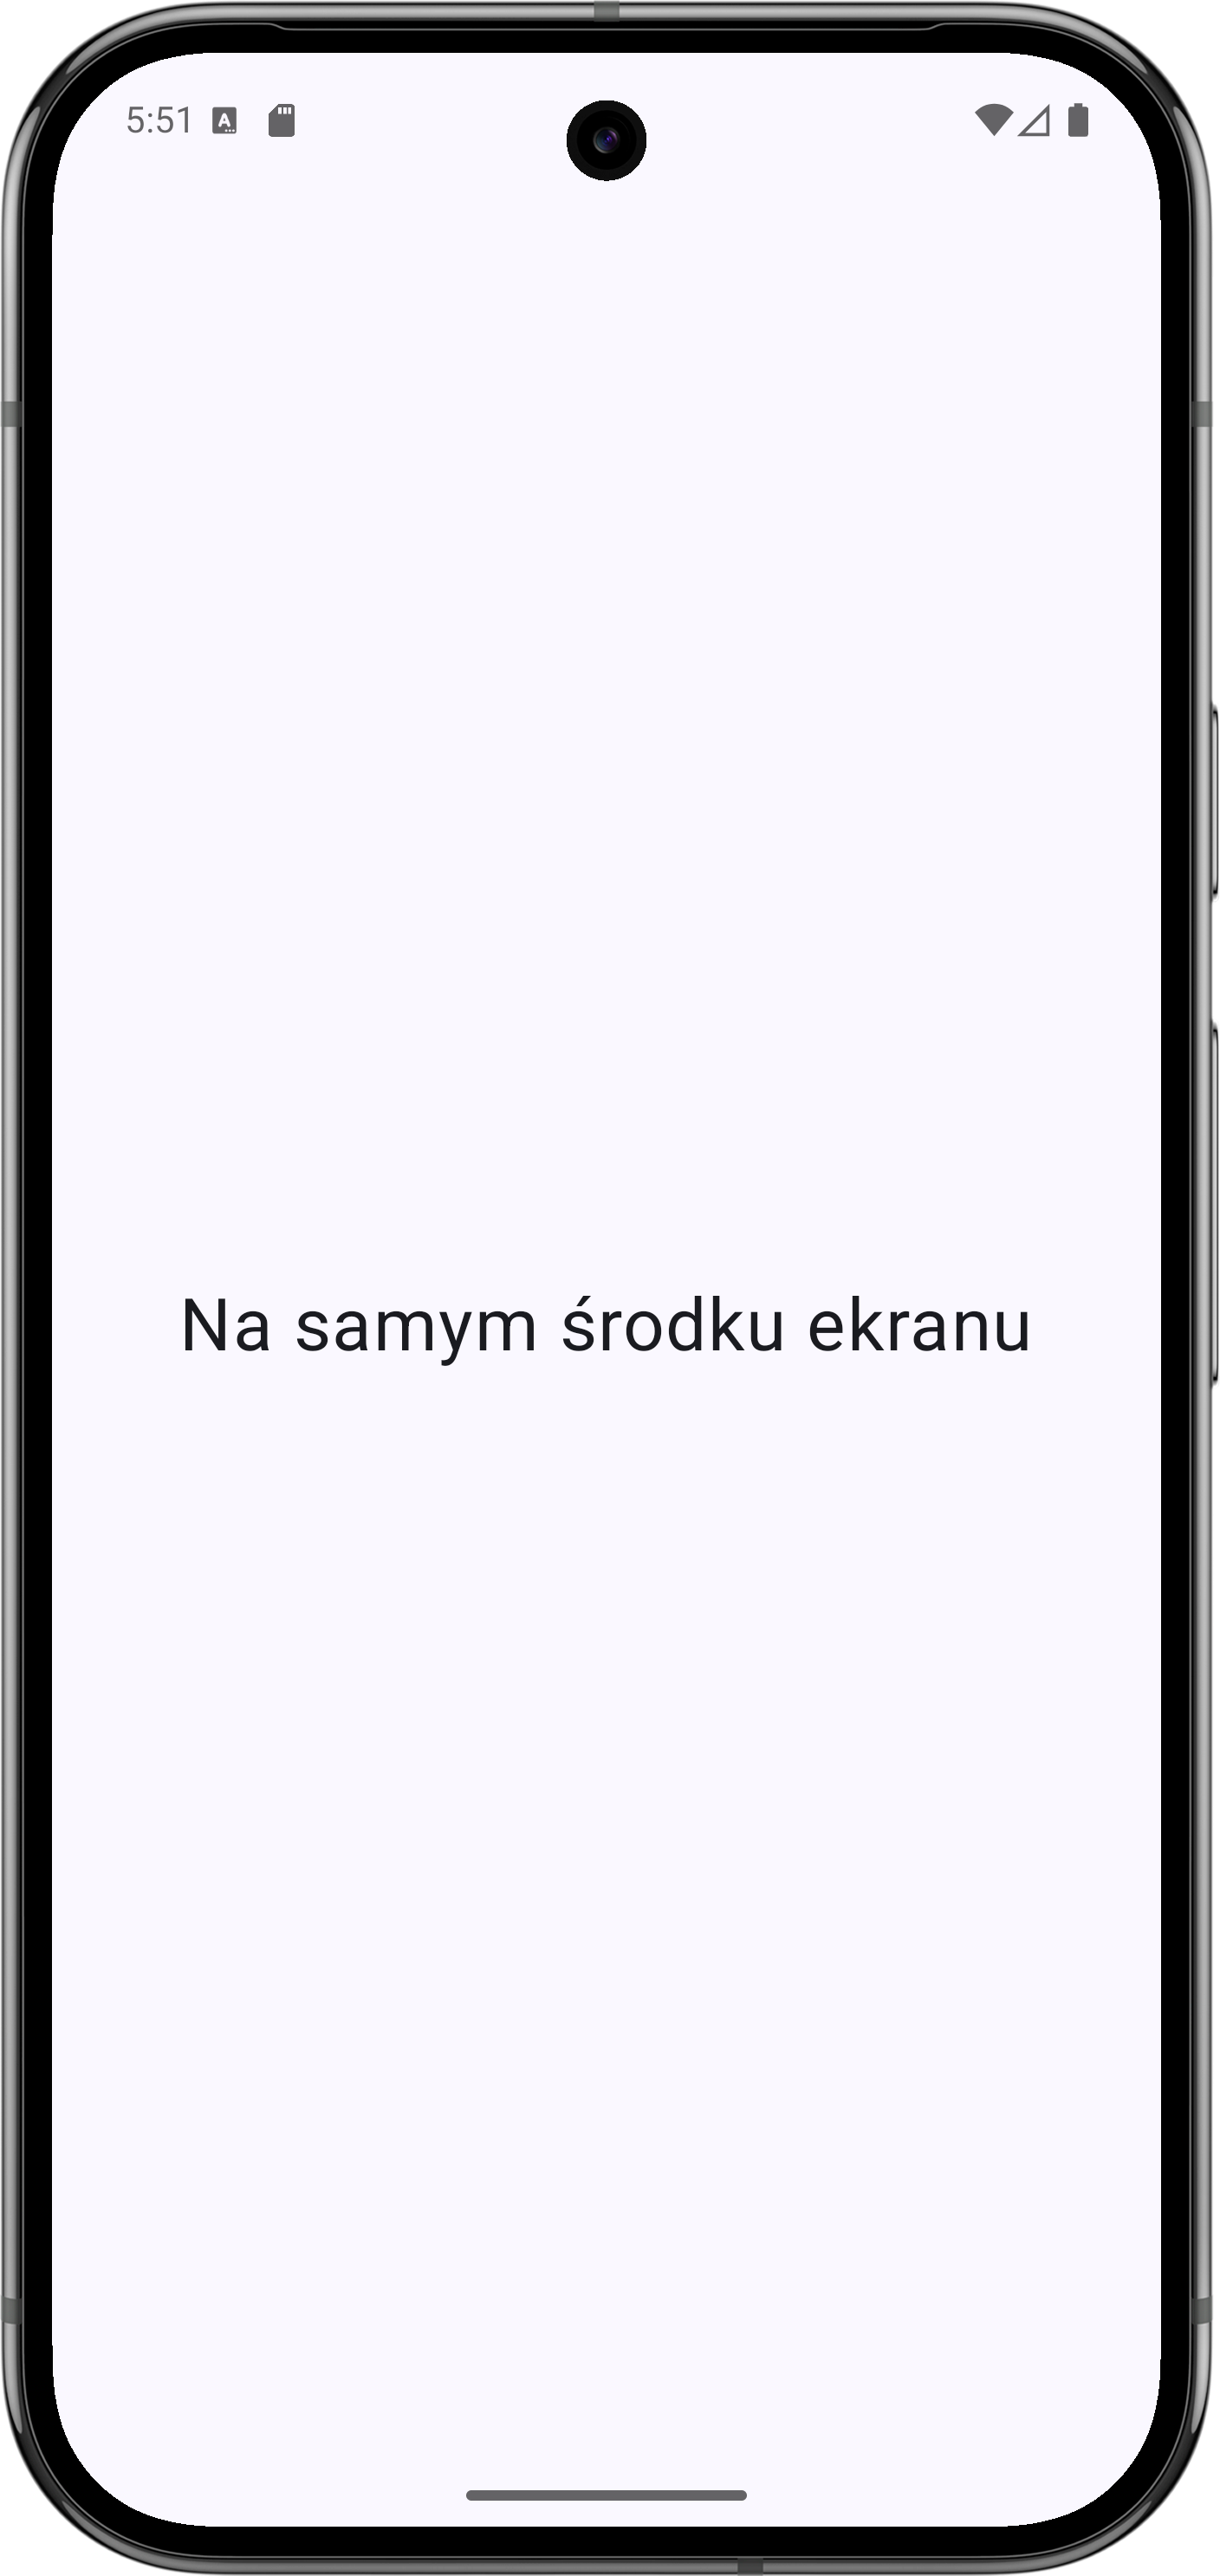
\includegraphics[width=0.25\textwidth]{fig/pum1-w09-arrangement_alignment.png}
    \caption{Wyśrodkowanie elementu w kontenerze}
    \label{fig:arrangement_alignment_viz}
\end{figure}

\section{Zarządzanie Stanem (State)}

Najtrudniejszą zmianą mentalną w Compose jest zrozumienie, czym jest stan i jak wpływa on na UI.

Wyobraź sobie, że interfejs użytkownika (UI) to \textbf{odbicie w lustrze}.
Jeśli jesteś niezadowolony z tego, co widzisz w lustrze (np. masz potargane włosy), nie próbujesz naprawiać samego lustra ani malować po jego powierzchni. Aby zmienić odbicie, musisz zmienić \textbf{obiekt stojący przed lustrem} (czyli uczesać włosy).

W tej analogii:
\begin{enumerate}
    \item \textbf{Lustro} to Framework (Compose). Jest ono nienaruszalne.
    \item \textbf{Odbicie} to Twój Ekran (UI). Jest tylko skutkiem, a nie przyczyną.
    \item \textbf{Obiekt przed lustrem} to \textbf{Stan} (Dane). To tutaj zachodzą zmiany.
\end{enumerate}

Równanie $UI = f(state)$ oznacza, że interfejs jest tylko i wyłącznie wizualną reprezentacją aktualnych danych. Nie można \textit{zmienić tekstu} na ekranie bezpośrednio; można jedynie zmienić zmienną (stan), a Compose (lustro) automatycznie zaktualizuje to, co widzi użytkownik.

W tym miejscu wprowadźmy pojęcia kompozycji i rekompozycji.
\begin{itemize}
    \item \textbf{Kompozycja (Composition)}: To proces, w którym Compose wykonuje Twoje funkcje \texttt{@Composable}, aby zbudować w pamięci opis (drzewo) interfejsu. To definicja UI nakarmiona aktualnymi danymi. Nie jest to jeszcze samo \textit{rysowanie} pikseli, a raczej tworzenie planu tego, co ma zostać narysowane.
    \item \textbf{Rekompozycja (Recomposition)}: To aktualizacja tego opisu. Gdy zmieniają się dane (stan), Compose wykonuje ponownie tylko niezbędne funkcje, aby dostosować drzewo UI do nowej rzeczywistości.
\end{itemize}

Jeśli zmieni się tylko jedna mała liczba w stanie, Compose nie przerysuje całego ekranu. Uruchomi ponownie (zrekomponuje) tylko te funkcje, które korzystają z tej konkretnej liczby. Reszta pozostanie nienaruszona.

\section{Anatomia Funkcji @Composable}

Skoro kompozycja to proces wykonywania funkcji \texttt{@Composable}, musimy zrozumieć, czym one właściwie są. Adnotacja \texttt{@Composable} zmienia typ funkcji w oczach kompilatora.

\begin{itemize}
    \item \textbf{Emisja UI, nie zwracanie wartosci}: Funkcje te zazwyczaj zwracają \texttt{Unit}. Ich celem nie jest zwrócenie obiektu widoku, ale \textbf{wyemitowanie} opisu interfejsu do drzewa kompozycji.
    \item \textbf{Kontekst wywołania}: Funkcję \texttt{@Composable} można wywołać \textbf{tylko} z innej funkcji \texttt{@Composable}. Tworzy to hierarchię wywołań, która startuje od metody \texttt{setContent} w Activity.
    \item \textbf{Zawartość}: Wewnątrz funkcji kompozycyjnej możemy:
    \begin{enumerate}
        \item Wywoływać inne funkcje \texttt{@Composable} (np. \texttt{Text}, \texttt{Column}).
        \item Używać standardowej logiki Kotlina (\texttt{if}, \texttt{for}, \texttt{when}) do sterowania tym, co zostanie wyemitowane.
        \item Zarządzać stanem (\texttt{remember}).
    \end{enumerate}
\end{itemize}

\begin{minted}[frame=single,framesep=10pt]{kotlin}
// Zwykła funkcja - zwraca String
fun formatName(name: String): String {
    return name.uppercase()
}

// Funkcja Composable - emituje UI
@Composable
fun Greeting(name: String) {
    // Możemy używać logiki
    if (name.isNotEmpty()) {
        // I wywoływać inne funkcje Composable
        Text("Witaj, ${formatName(name)}")
    }
}
\end{minted}

\section{Przechowywanie Stanu}

Funkcje w Kotlinie są z natury bezstanowe – gdy funkcja się kończy, jej zmienne lokalne znikają. Jak więc zachować np. stan licznika między odświeżeniami ekranu?

\begin{minted}[frame=single,framesep=10pt]{kotlin}
@Composable
fun Counter() {
    // 1. mutableStateOf tworzy obserwowalny stan (startujemy od 0)
    // 2. remember sprawia, że ta zmienna "przeżyje" rekompozycję
    var count by remember { mutableStateOf(0) }

    Button(onClick = { count++ }) { // Zmiana stanu wyzwala rekompozycję
        // Podczas rekompozycji, Compose widzi nową wartość count
        Text("Kliknięto $count razy") 
    }
}
\end{minted}

Tutaj wchodzą dwaj gracze:

\begin{enumerate}
    \item \texttt{mutableStateOf(value)}: To specjalne \textit{pudełko} na dane, które jest \textbf{obserwowalne}. Gdy zmienisz zawartość tego pudełka (np. \texttt{count.value++}), Compose dostaje sygnał: \textit{"Musisz odświeżyć wszystkich, którzy na to patrzą"}.
    \item \texttt{remember \{ ... \}}: To instrukcja dla kompilatora: \textit{Zapisz ten obiekt w pamięci podręcznej obok drzewa UI}. Gdy funkcja \texttt{Counter} zostanie wywołana ponownie (rekompozycja), \texttt{remember} odda nam zachowaną wcześniej wartość, zamiast tworzyć nową (zresetowaną do zera).
\end{enumerate}

Bez \texttt{remember}, przy każdym kliknięciu funkcja \texttt{Counter} startowałaby od nowa z wartością 0. Bez \texttt{mutableStateOf}, zmiana zmiennej nie dałaby sygnału do odświeżenia ekranu (interfejs byłby martwy).

Mimo że \texttt{remember} działa podczas rekompozycji, ma jedną wadę: \textbf{zapomina wszystko przy zmianie konfiguracji} (np. obrót ekranu, zmiana języka, tryb ciemny). Wtedy cała aktywność jest niszczona i tworzona od nowa, a pamięć podręczna \texttt{remember} jest czyszczona.

Aby zachować stan nawet po \textit{śmierci} i odrodzeniu się aktywności (lub procesu), używamy \texttt{rememberSaveable}. Pod maską wykorzystuje on mechanizm \texttt{Bundle} (ten sam co w \texttt{onSaveInstanceState} z klasycznego Androida).

\begin{minted}[frame=single,framesep=10pt]{kotlin}
@Composable
fun ResilientCounter() {
    // rememberSaveable przeżyje obrót ekranu!
    var count by rememberSaveable { mutableStateOf(0) }

    Button(onClick = { count++ }) {
        Text("Kliknięto $count razy")
    }
}
\end{minted}

Dla prostych typów (Int, String, Boolean) działa to automatycznie. Dla własnych obiektów musimy dostarczyć tzw. \texttt{Saver} (np. implementując \texttt{Parcelable} i używając \texttt{@Parcelize}).

\subsection{Składnia: = vs by}
Często spotkamy się z dwoma zapisami stanu:

\begin{minted}[frame=single,framesep=10pt]{kotlin}
// 1. Przypisanie (=)
val nameState = remember { mutableStateOf("Jan") }
Text(text = nameState.value) // Musimy pisać .value

// 2. Delegacja (by)
var name by remember { mutableStateOf("Jan") }
Text(text = name) // Używamy jak zwykłej zmiennej
\end{minted}

Słowo kluczowe \texttt{by} (delegacja właściwości) \textit{odpakowuje} dla nas stan.
\begin{itemize}
    \item Przy \texttt{by}, zmienna \texttt{name} jest typu \texttt{String} (kompilator ukrywa \texttt{State} pod spodem). Aby zmienić wartość, piszemy \texttt{name = "Ewa"}.
    \item Przy \texttt{=}, zmienna \texttt{nameState} jest typu \texttt{MutableState<String>}. Aby zmienić wartość, musimy pisać \texttt{nameState.value = "Ewa"}.
\end{itemize}
Używanie \texttt{by} wymaga importów (które czasami nie są dodawane automatycznie przez IDE):
\texttt{import androidx.compose.runtime.getValue}
\texttt{import androidx.compose.runtime.setValue}

\section{Wzorzec State Hoisting}

Aby komponenty były wielokrotnego użytku i łatwe w testowaniu, stosujemy wzorzec \textbf{State Hoisting} (wynoszenie stanu w górę). Polega on na tym, że komponent nie zarządza swoim stanem wewnętrznie, ale otrzymuje go od rodzica.

Cechy komponentu \textbf{Stateless} (bezstanowego):
\begin{enumerate}
    \item Otrzymuje stan przez parametr (np. \texttt{value: String}).
    \item Zgłasza zdarzenia przez lambdę (np. \texttt{onValueChange: (String) -> Unit}).
\end{enumerate}

\begin{minted}[frame=single,framesep=10pt]{kotlin}
// Komponent Stateful (zarządza stanem - trudniejszy do testowania i reużycia)
@Composable
fun HelloScreen() {
    var name by remember { mutableStateOf("") }
    HelloContent(name = name, onNameChange = { name = it })
}

// Komponent Stateless (czysta funkcja UI)
@Composable
fun HelloContent(name: String, onNameChange: (String) -> Unit) {
    Column {
        Text("Cześć $name")
        TextField(
            value = name,
            onValueChange = onNameChange
        )
    }
}
\end{minted}

Dzięki temu \texttt{HelloContent} jest niezależny od tego, skąd pochodzi stan (może to być \texttt{remember}, \texttt{ViewModel}, czy stała z testu).
Wzorzec ten promuje \textbf{Unidirectional Data Flow} (Jednokierunkowy Przepływ Danych):
\begin{itemize}
    \item Dane płyną \textbf{w dół} (od rodzica do dziecka).
    \item Zdarzenia płyną \textbf{w górę} (od dziecka do rodzica).
\end{itemize}

\begin{figure}[h]
    \centering
    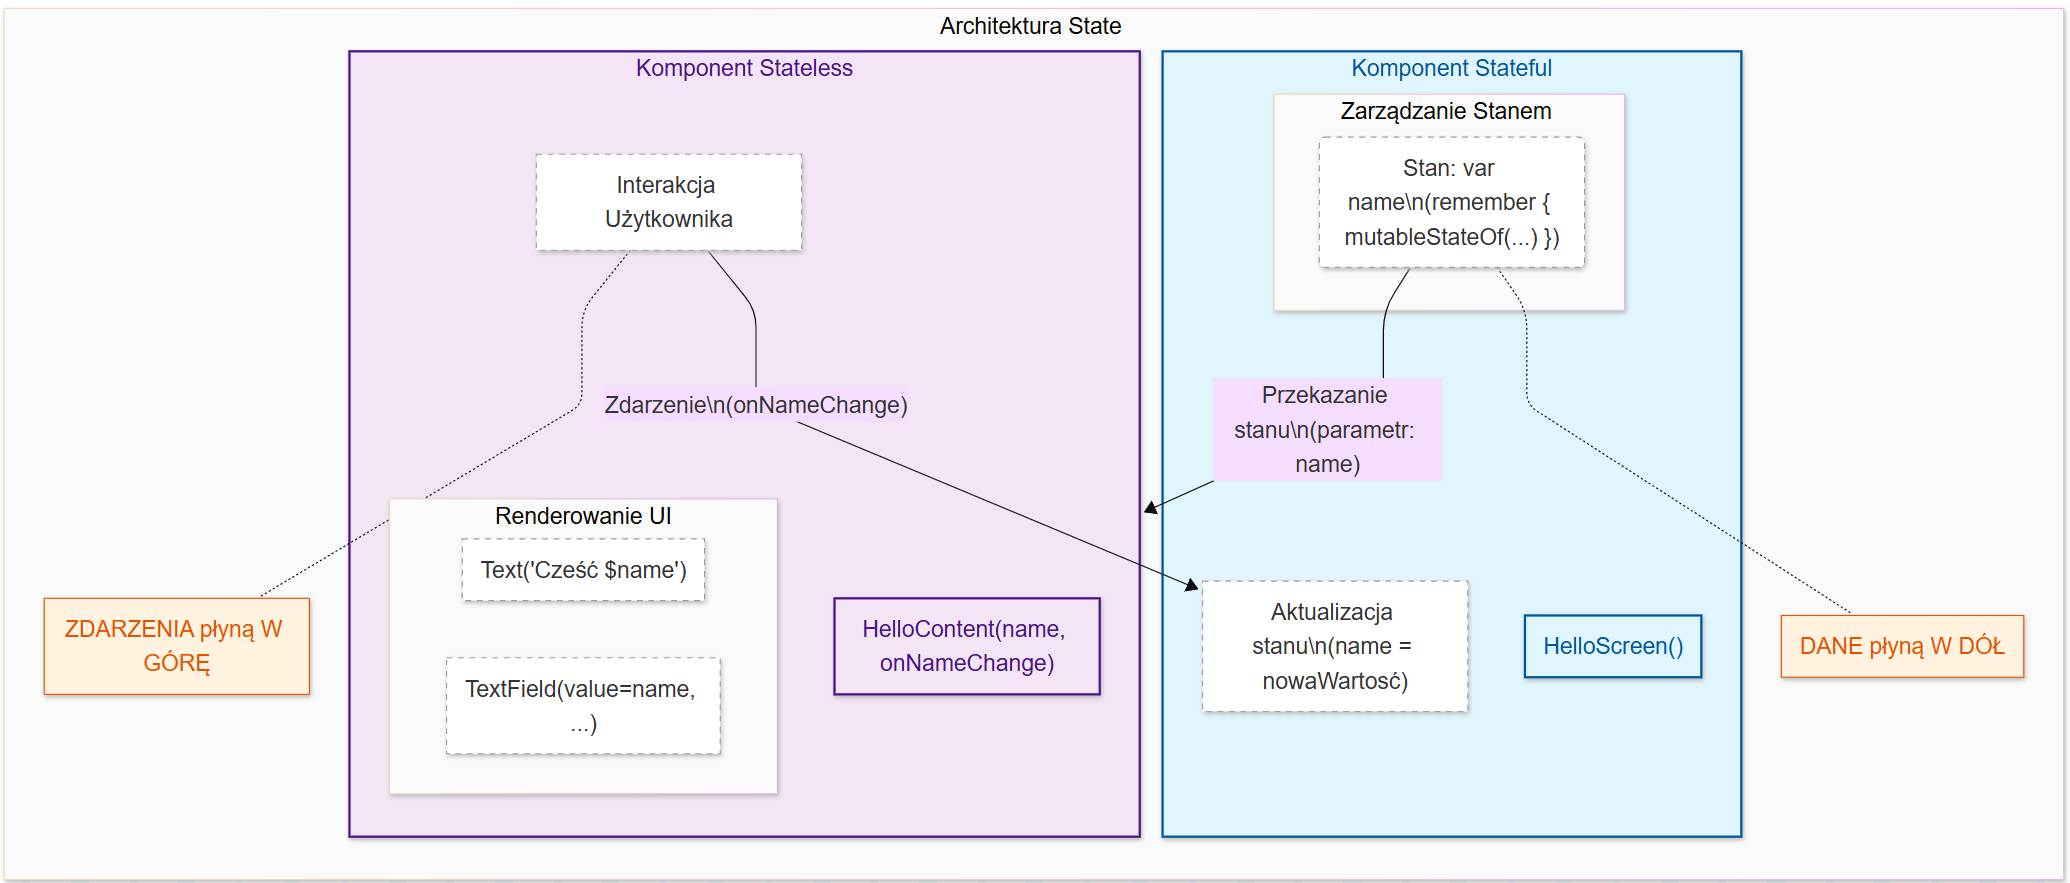
\includegraphics[width=1.0\textwidth]{fig/pum1-w09-state_hoisting.png}
    \caption{Wzorzec State Hoisting}
    \label{fig:pum1-w09-state-hoisting}
\end{figure}